\chapter{Results}
\label{ch:result}
The tool is setup on a 64-bit Ubuntu 20.04 LTS, 7.7 GB of RAM and 8 Core Intel(R) Core(TM) i5-8250U CPU @ 1.60GHZ. A Total of 35 smart contracts are tested with 6 different sets of \{Invocations, Path length\}. We have tested the tool on 1 and 2 invocations with path length 10, 20 and 40 respectively for each of the mentioned invocations.
The result of the tool for 1 invocation and sets of path length is shown in the Chart 1.\\
\begin{center}
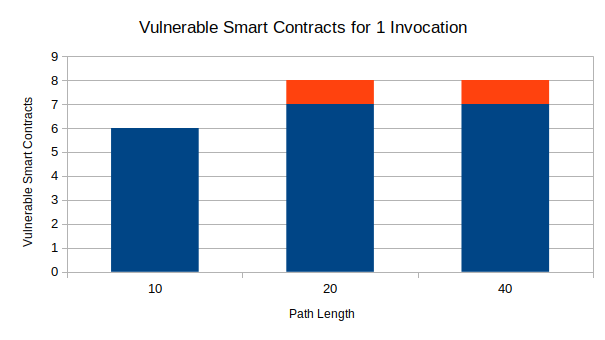
\includegraphics[width= 15cm]{images/51.png}

    Chart 1
\end{center}
A total of 6 smart contracts are flagged as vulnerable in the setup with 1 invocation and path length equals to 10. A total of 7 smart contracts are flagged as vulnerable in the setup with 1 invocation and path length equals to 20. Out of those 7 smart contracts. 1 smart contract is false positive. The result with 1 invocation and path length 40 path length is same as the 1 invocation and 20 path length.\\
The result of the tool for 2 invocations i s shown in the Chart 2. 
\begin{center}
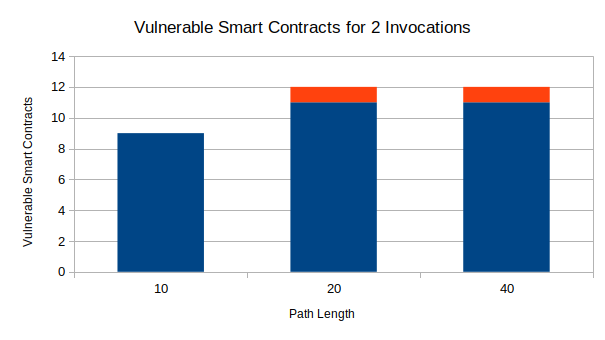
\includegraphics[width = 15cm]{images/52.png}
Chart 2
\end{center}
\noindent A total of 9 smart contracts are flagged as vulnerable in the setup with 2 invocation and path length equals to 10. A total of 11 smart contracts are flagged as vulnerable in the setup with 2 invocation and path length equals to 20. Out of those 11 smart contracts, 1 smart contract is false positive. The result with 2 invocation and path length 40 path length is also the same as the 2 invocation and 20 path length. \\

\begin{center}
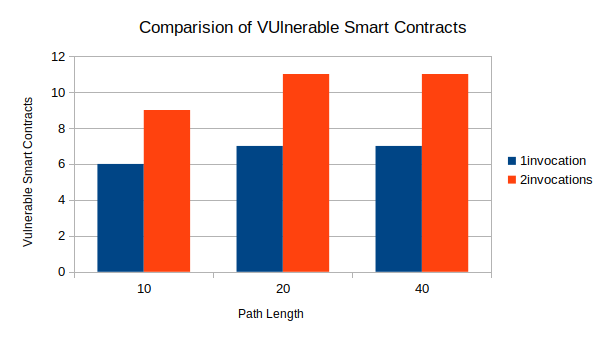
\includegraphics[width= 16cm]{images/53.png}
Chart 3
\end{center}
The 2 invocation setup was able to find more vulnerable contract which otherwise was left by the 1 invocation setup. This was expected as we have explained in Symbolic Execution Phase of the Dos Tool. Also with the increase in number of path length the tool was able to traverse path more deeply and explore more vulnerabilities if present. A comparison chart with different invocation setup and path length is shown in Chart 3.\\

\section*{About the False Positive Case}
The false positive case is for the vulnerability of unbounded loop condition. We have assumed that the symbolic value can take any value. For the example consider this value as the integer value. Now the integer type variable have different ranges based on the type of integer in solidity. For example solidity have signed and unsigned integer of different sizes. The range varies from 8 bit number to 256 bit number with keywords : unint8 to unint256 and int8 to int256. An unsigned integer uint32 has a range from 0 to 2**32 - 1\cite{integer}. \\
But SMT solver on symbolic expressions yield same result of all different ranges of integer value in the loop condition and we have given the range limit of 256 bit number for the SMT Solver. We need to know different range of integers which with the current tool is not possible to determine and the SMT will overestimate paths based on our current setup. The smart contract which gives false positive looks like below:
\begin{Verbatim}[numbers=left,xleftmargin=5mm]
    function nameFilter(string _input)
        returns(bytes32)
    {
        uint256 _length = _temp.length;
        require (_length <= 32 && _length > 0);
        for (uint256 i = 0; i < _length; i++)
        {
            //some code
        }
    }
\end{Verbatim}
Although the \emph{\_input} length is symbolic since the string is symbolic. Its length is limited by the line number 5 of the code. But the SMT will return satisfiable for the Symbolic expression in the loop condition at line 6. These limitations based on integer size or checks as performed in the above code are falsely interpreted as vulnerable contracts by the tool.
